\PassOptionsToPackage{unicode,pdfusetitle}{hyperref}
\PassOptionsToPackage{hyphens}{url}
\PassOptionsToPackage{dvipsnames}{xcolor}

\documentclass[english,a4paper]{article}

\usepackage{geometry}

% Font settings
\usepackage[T1]{fontenc}
\usepackage{lmodern}
\usepackage{amssymb,amsmath,amsthm,mathtools}
\usepackage{textcomp}
\usepackage{csquotes}
\usepackage{babel}
\usepackage{upquote}

\usepackage[textsize=footnotesize]{todonotes}

\usepackage{microtype}
\UseMicrotypeSet[protrusion]{basicmath} % disable protrusion for tt fonts

% Colors
\usepackage{xcolor}

% Hyperlinks, urls, etc
\usepackage{xurl}

\usepackage{hyperref}
\hypersetup{
  colorlinks = true,
  breaklinks = true,
  linkcolor  = black,
  filecolor  = MidnightBlue,
  citecolor  = MidnightBlue,
  urlcolor   = MidnightBlue
}

\usepackage{cleveref}

% Floats
\usepackage{graphicx}
\usepackage{booktabs}
\usepackage{caption}
\usepackage{subcaption}

% Algorithms
\usepackage{algorithm,algpseudocode}

% Title Page
\usepackage[]{authblk}
\renewcommand\Affilfont{\itshape\small}

\setlength{\emergencystretch}{3em} % prevent overfull lines

% operators
\DeclareMathOperator*{\argmax}{arg\,max}
\DeclareMathOperator*{\argmin}{arg\,min}
\DeclareMathOperator{\E}{E}
\DeclareMathOperator{\var}{Var}
\DeclareMathOperator{\cov}{Cov}
\DeclareMathOperator{\tr}{tr}
\DeclareMathOperator{\diag}{diag}
\DeclareMathOperator{\range}{range}
\DeclareMathOperator{\nullspace}{null}
\DeclareMathOperator{\rank}{rank}
\DeclareMathOperator{\card}{card}
\DeclareMathOperator{\sign}{sign}
\DeclareMathOperator{\st}{S}
\DeclareMathOperator{\normal}{Normal}
\DeclareMathOperator{\fnormal}{FoldedNormal}
\DeclareMathOperator{\bernoulli}{Bernoulli}
\DeclareMathOperator{\erf}{erf}
\DeclareMathOperator{\mse}{MSE}
\DeclareMathOperator{\risk}{R}
% \DeclareMathOperator{\I}{I}
% \DeclareMathOperator{\T}{}
%
% \DeclareMathSymbol{\phi}{\mathalpha}{operators}{0}
\DeclareMathOperator{\pdf}{\phi}
\DeclareMathOperator{\cdf}{\Phi}
% commands
% \newcommand{\vec}{\vectorsym}
% \newcommand{\mat}{\matrixsym}
\renewcommand{\vec}{\boldsymbol}
\newcommand{\mat}{\boldsymbol}
\newcommand*\du{\mathop{}\!\mathrm{d}}
% \newcommand{\T}{\mathsf{T}}
\newcommand{\T}{\intercal}
\newcommand{\ones}{\boldsymbol{1}}
% \newcommand{\T}{\intercal}
% \newcommand{\T}[1]{{1}^{\mathsf{T}}}
\newcommand{\ind}[1]{\operatorname{I}_{#1}}

% environments
\theoremstyle{plain}
\newtheorem{theorem}{Theorem}[section]
\newtheorem{corollary}{Corollary}[theorem]
\newtheorem{lemma}{Lemma}[section]
\newtheorem{proposition}{Proposition}[section]

\theoremstyle{definition}
\newtheorem{definition}{Definition}[section]
\newtheorem{example}{Example}[section]

\theoremstyle{remark}
\newtheorem{remark}[theorem]{Remark}

\newcommand{\todojl}[1]{\todo[color=green!40]{#1}}



% title block
\title{Standardization and Regularization}
\author[1,*]{Johan Larsson}
\affil[1]{Department of Statistics, Lund University}
\affil[*]{Corresponding author:
  \href{mailto:johan.larsson@stat.lu.se}{\nolinkurl{johan.larsson@stat.lu.se}}
}
\date{\today}

% bibliography
\usepackage[style=alphabetic]{biblatex}
\addbibresource{normreg.bib}

\begin{document}

\maketitle

\section{Introduction}

When the data you want to model is high-dimensional, that is, the number of features \(p\) exceed the number of observations \(n\), it is impossible to apply classical statistical models such as standard linear regression since the design matrix \(\mat X\) is no longer of full rank. A common remedy to this problem is to \emph{regularize} the model by adding a term to the objective function that punishes models with large coefficients (\(\vec\beta\)). If we let \(h(\vec\beta; \mat X, \vec y)\) be the original objective function---which when minimized improves the model's fit to the data (\(\mat X, \vec y\))---then
\[
  f(\beta_0, \vec\beta; \mat X, \vec y) = h(\beta_0, \vec\beta; \mat X, \vec y) + g(\vec\beta)
\]
is a composite function within which we have added a penalty term \(g(\vec\beta)\).
In contrast to \(h\), this penalty depends only on the coefficients (\(\vec{\beta}s\)).
The intercept, \(\beta_0\), is not typically penalized.

Some of the most common penalties are the \(\ell_1\) and \(\ell_2\) penalties, that is \(g(\vec\beta) = \lVert \vec\beta \rVert_1\) or \(g(\vec\beta) = \lVert \vec\beta \rVert_2^2/2\)\footnote{Division by two in this case is used only for convenience.}, which, if \(h\) is the standard ordinary least-squares objective, represent lasso and ridge (Tikhonov) regression respectively.
Other common penalities include SLOPE, MCP, hinge loss (used in support vector machines) and SCAD.
Many of these penalities---indeed all of the previously mentioned ones---shrink coefficients in proportion to their sizes.

% TODO: Maybe say something about ℓ₀ (best subset) regularization

The issue with this type of shrinkage is that it is typically sensitive to the scales and locations of the features in \(\mat X\).
A common remedy is to \emph{normalize} the features before fitting the model by translating and dividing each column by respective translation and scaling factors.
For some problems, such factors may arise naturally from knowledge of the problem at hand.
A researcher may for instance have collected data on coordinates within a limited area and know that the coordinates are measured in meters.
Often, however, these scaling and location factors must be estimated from data.
The most popular choices for this type of scaling are based only on the marginal distributions of the features.
Some types of normalization, such as that applied in the adaptive lasso\footnote{The adaptive lasso typically uses ordinary least square estimates of the regression coefficients to scale the features with.}, however, are based on the conditional distributions of the features and the response.
After fitting the model, the estimated coefficients are then usually returned to their original scale.

Another reason for normalizing the features is to improve the performance and stability of optimization algorithms used to fit the model.
We will not cover this aspect in this paper, but note that it is an important one.

\section{Theory}

\subsection{Terminology}

We begin with a section on terminology in order to avoid confusion regarding the varied use of key terms in the field. The terms \emph{scaling}, \emph{standardization}, and \emph{normalizaton} are for instance used interchangeably in the literature.

Here, we define \emph{normalization} as the process of translating and scaling the feature matrix.
More formally, we introduce a scaling matrix \(\mat S = \diag(s_1, s_2, \dots, s_p)\), with \(s_j > 0\) and an \(n \times p\) large translation matrix \(\mat T\) where \(t_{ij} = t_{kj}\) for all \(i,k \in [n]\). Then \(\tilde{\mat X} = (\mat X - \mat T) \mat S^{-1}\) is the normalized design matrix.

Some authors use \emph{standardization} or \emph{scaling} to refer to this procedure, but in this paper we will define scaling only as defined above and standardization as the particular case in \Cref{tab:normalization-types}.

\begin{table}[hbt]
  \centering
  \caption{Common ways to normalize a matrix of features.}
  \label{tab:normalization-types}
  \begin{tabular}{lll}
    \toprule
    Normalization    & Translation (\(t_j\))              & Scaling (\(s_j\))                                         \\
    \midrule
    Standardization  & \(\frac{1}{n}\sum_{i=1}^n x_{ij}\) & \(\sqrt{\frac{1}{n}\sum_{i=1}^n (x_{ij} - \bar{x}_j)^2}\) \\
    \addlinespace
    Min--Max         & \(\min_i(x_{ij})\)                 & \(\max_i(x_{ij}) - \min_i(x_{ij})\)                       \\
    \addlinespace
    Unit Vector (L2) & 0                                  & \(\sqrt{\sum_{i=1}^n x_{ij}^2}\)                          \\
    \addlinespace
    Max Abs          & 0                                  & \(\max_i(|x_{ij}|)\)                                      \\
    \addlinespace
    Adaptive Lasso   & 0                                  & \(\beta_j^\text{OLS}\)                                    \\
    \bottomrule
  \end{tabular}
\end{table}

\subsection{The Lasso}

As a initial example of this, let us take \(h\) to be the lasso objective, where \(f\) is the ordinary least-squares objective and \(h\) the \(\ell_1\) norm and consider a one-dimensional problem, that is, the composite objective is
\[
  \frac{1}{2} \sum_{i=1}^n(y_i - \beta_0 - \vec{x}^T_i \vec\beta)^2 + \lambda \lvert \vec\beta \rvert.
\]

% TODO: Convert this into a theorem about elastic net instead.
\begin{proposition}
  If \(\mat X^\T \mat X\) is diagonal, then
  \[
    \hat{\beta}_j = \frac{s_j\softthreshold\big((\vec x_j - \vec{1}t_j)^\T\vec{y}; s_j\lambda\big)}{\lVert \vec x_j - \vec{1}t_j\rVert_2^2} \text{ for all } j \in [p],
  \]
  where \(\softthreshold(\beta; \lambda) = \sign(\beta)\max\big(\lvert \beta \rvert - \lambda, 0\big)\) is the \emph{soft thresholding operator}.
\end{proposition}
\begin{proof}
  The KKT stationarity condition for the normalized lasso problem is
  \[
    \vec{0} \in \tilde{\mat{X}}^\T(\tilde{\mat{X}}\vec{\beta} - \vec{y}) + \lambda g,
  \]
  where \(g\) is the subgradient of the \(\ell_1\) norm.
  If \(\mat{X}^\T\mat{X}\) is diagonal, then this condition resolves into \(p\) piecewise conditions given by
  \[
    0 \in \tilde{\vec{x}}_j^\T\tilde{\vec{x}}_j\beta_j - \tilde{\vec{x}}_j^\T\vec{y} + \lambda g \quad \forall\, j \in [p].
  \]
  The subdifferential of the \(\ell_1\) norm is \([-1, 1]\), that is, \(g \in [-1, 1]\), and it is well-known that the solution to the equation above is
  given by
  \[
    \frac{\softthreshold(\tilde{\vec{x}}_j^\T \vec{y}; \lambda)}{\lVert \tilde{\vec{x}}_j\rVert_2^2} =
    \frac{s_j\softthreshold\big((\vec{x}_j - \vec{1}t_j)^\T\vec{y}; s_j\lambda\big)}{\lVert \vec{x}_j - \vec{1}t_j\rVert_2^2}.
  \]
\end{proof}

\subsection{Binary Data}

The validity of normalization implicitly assumes that we can put the features in our design on an identical, or at least similar, scale. For data coming from continuous variables, this assumption is often tenable. But it is harder to justify when faced with a mix of continuous and binary data.

First, we need to determine how to match a flip of the binary variable (a one unit change) with an equivalent amount of change in the continuous variable. There are several possibilities, and none are unequivocally correct. For the sequel, we will assume that moving two standard deviations on the continuous variable is equivalent to flipping the binary variable. If the continuous variable comes from a normal distribution, this means that having the class represented by the binary feature or not is equivalent to being in the lower versus upper 16\% of the distribution of the continuous variable. We argue that this is a reasonable way to match these variables---one which has support elsewhere~\parencite{gelman2008}.

Let us start by assuming that we have a two-dimensional problem and that \(x_{i1} \sim \bernoulli(p)\) and \(x_{i2} \sim \normal(0, 1)\) with no dependence between either the features or the observations. When \(q = 0.5\), the classes are completely balanced, and the population standard deviations become 0.5 and 1 for \(\vec{x}_2\) and \(\vec{x}_1\) respectively. And if we choose to normalize with mean and standard deviation, then, after standardization, values for \(\vec{x}_2\) will lie between 0 and 2, with a standard deviation of 1. For \(\vec{x}_2\), 69\% of the values will lie between an equally spaced range, -1 to 1, and the standard deviation will of course also be 1. If the true model is \(y = \mat{X}\vec{\beta}\) and \(\beta = [1,1]^\T\), then shrinkage will be applied equally across the coefficients of the two features.

\begin{figure}[htpb]
  \centering
  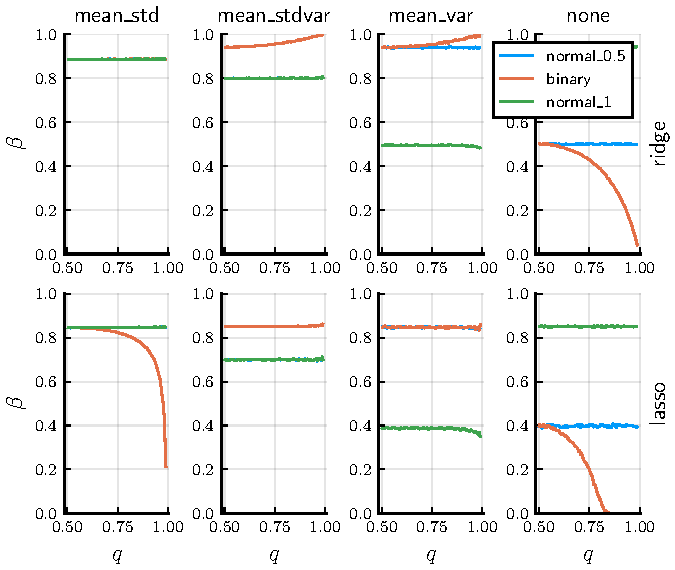
\includegraphics[]{plots/lasso_ridge_twodim.pdf}
  \caption{%
    Comparison between lasso and ridge estimators for a two-dimensional problem where one feature is generated from \(\bernoulli(q)\) and the other from \(\normal(0, 0.5)\). The ridge estimator is unaffected by \(q\), but the lasso estimator is not.
  }
  \label{fig:lasso-ridge-comparison}
\end{figure}

\begin{figure}[htpb]
  \centering
  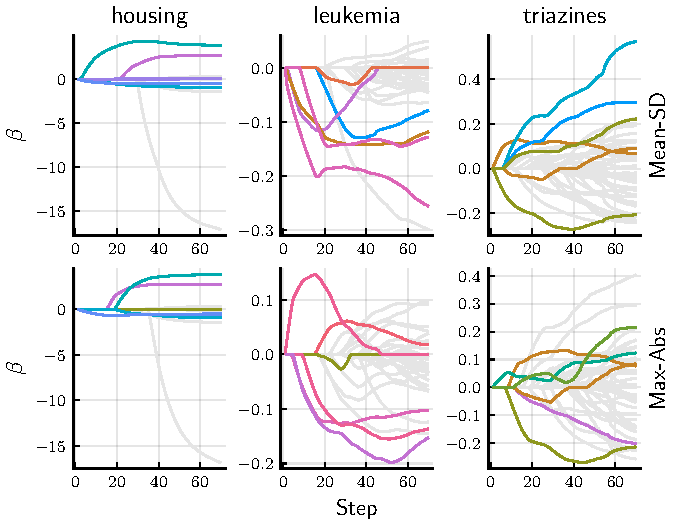
\includegraphics[]{plots/realdata_paths.pdf}
  \caption{%
    A display over the first predictors selected by the lasso for each type of normalization. Each panel shows the union of the first five predictors picked by either type of normalization.
  }
  \label{fig:realdata-paths}
\end{figure}

\subsection{Maximum Absolute Value Scaling}

In \Cref{fig:maxabs-n} we show how the coefficient corresponding to the Normally distributed feature shrinks as the number of observation \(n\) increases.

\begin{figure}[htpb]
  \centering
  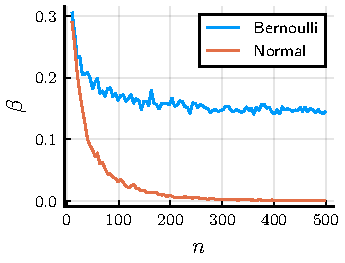
\includegraphics[]{plots/maxabs_n.pdf}
  \caption{%
    Effects of maximum absolute value scaling.
  }
  \label{fig:maxabs-n}
\end{figure}

\section{To Do}

\begin{itemize}
  \item Use homotopy path algorithm to express upcoming critical \(\lambda\) values as a function oDiscussing whether or not this is a reasonable transformation that indeed should place these variables on a similar scale is f the scaling of the features.
  \item Solve two-dimensional ridge regression problem with correlation to examine the effects of correlation between a binary and a continuous variable.
  \item Solve a two-dimensional lasso problem, without correlation, to observe the relative effect of standard deviation.
  \item Use Fisher–Tippett–Gnedenko theorem to say something about the effect of max-abs-scaling when used with gaussian and bernoulli variables.
  \item Consider the relationship to adaptive lasso.
  \item Consider other penalties to generalize and appeal to a broader audience: MCP, SCAD, hinge loss.
\end{itemize}

\section{Insights}

\begin{itemize}
  \item Rare traits (especially in binary data), will ``never'' be selected
  \item Outliers can cause variables to not be selected.
  \item Scaling with maximum absolute value means that for a Gaussian variable, the importance of a variable decrease with the number of samples (since the change of encountering a high value increases).
\end{itemize}

\section{Open Questions}

\begin{itemize}
  \item What effect does standardization have when it is used in the presence of dummy variables?
  \item Should dummy variables be standardized?
  \item In which situations is standardization of type x useful? What about type y?
  \item Is this only a problem for simpler models? I.e., does it matter for neural networks, for instance? Probably not.
  \item Adaptive lasso can be seen as a type of pre-processing. How does it compare? Does it fix the problems here?
  \item We standardize unconditionally, but interpret regression coefficients conditionally
  \item Can we quantify how strong a given feature's RMSE needs to be for it to be selected?
  \item How is prediction performance affected by this?
  \item How is false discovery rate affected by this?
  \item How is cross-validation affected by this?
  \item Can we mitigate the effect through stratification of the features?
  \item Can we mitigate the effect through some type of normalization?
\end{itemize}

\printbibliography

\end{document}
